% forecast
    % overall performance
    This section details the observable performance of R.F.I.D. following its design, assembly and testing.
    Of the highest concern is the performance of the power supply functional block \DIFdelbegin \DIFdel{, }\DIFdelend because it corresponds to the only quantitative specification. As such, this section will describe the power supply block first.
    Because the Local Storage and Time Keeper functional blocks share three technical specifications, they have been grouped together.
    The printed circuit board will be discussed lastly for a very brief description of its functioning.

\subsection{Power Supply}
% RELEVANT SPECS:
% DC-DC converter supplies 3.3V DC ±10% with a maximum ripple of 200mVpp and capable of at least 200mA
The specifications for the power supply were tested by quantitative measurements.  Prior to measuring for specifications, the output of the buck converter circuit was bypassed to H3 by placing a SPC02SYAN jumper between pins 1 and 4 of JP1, so as to test the Power Supply block independently from the rest of R.F.I.D. A ROX3SJ12R resistor with a nominal resistance of 12$\ohm{\pm}$5\% and a power rating of 3W was also placed between pins 1 and 4 of H3 to act as a test load between the output of the buck converter and ground. This test load was measured at 12.3$\ohm$ prior to its placement. All DC measurements were performed with a CSI2010 multimeter, while AC measurements were performed with a Tektronix MSO2014 oscilloscope paired with PVP2150 passive oscilloscope probes set to 10x attenuation.

First, the power supply's DC output voltage and output current capability were tested. An Adafruit 2011 battery was inserted \DIFdelbegin \DIFdel{to }\DIFdelend \DIFaddbegin \DIFadd{into battery connector }\DIFaddend CON1 to supply a 3.7VDC source to the input of the buck converter circuit. The buck converter's DC output voltage was then measured across the test load as 3.33VDC, which is 0.9\% greater than 3.3VDC, and well within the allowed 3.3VDC$\pm$10\%. With a 3.3VDC output voltage, and a resistance of 12.3$\ohm$, the output current was calculated via Ohm's \DIFdelbegin \DIFdel{Law }\DIFdelend \DIFaddbegin \DIFadd{law }\DIFaddend as 271mA, which meets and exceeds the specification for the power supply's output current capability. At this point, only the output voltage ripple was left for the measurement and verification of the project's power supply specifications.

%he DC and AC components of the buck converter's output voltage were measured separately by placing a test load between 

Next, the output voltage ripple was tested via an AC voltage measurement across the test load, with the same setup as used for prior measurements. The oscilloscope probes, while connected to channel one of the oscilloscope, were placed between the buck converter's output and ground, with the test load still in place. Since only the AC component, or ripple, of the output voltage was being measured, the oscilloscope was set to AC coupling to block the DC component of the voltage being measured. Since this step eliminated the DC voltage from the measurement, the y-axis scale could be decreased so as to obtain a visible and accurate measurement of the voltage ripple. The oscilloscopes horizontal scale was then set to 400$\mu$s per division, while the vertical scale was set to 0.05 per division. The measured ripple voltage is shown in Figure~\ref{fig:voltage_ripple}.

\begin{figure}[H]
    \centering
    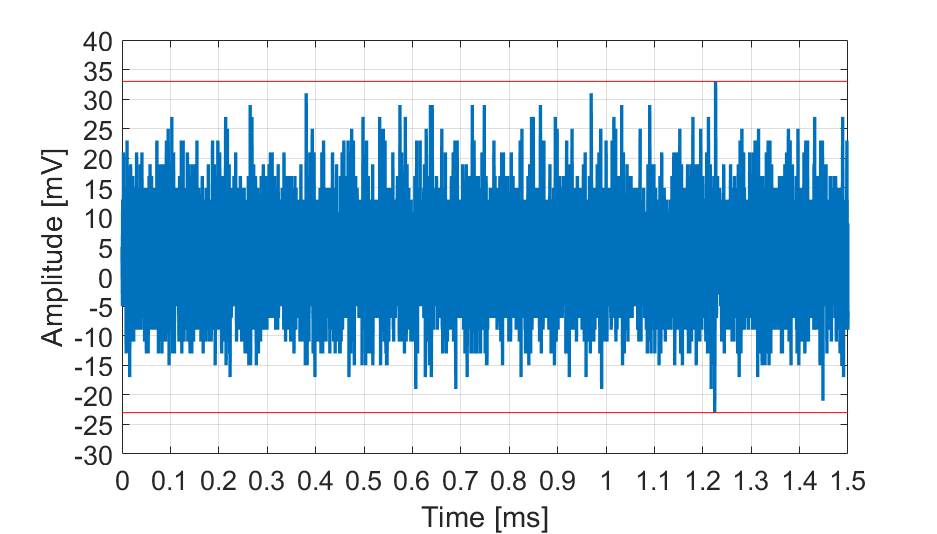
\includegraphics[width=1\textwidth]{Figures/5_results/supply1_polished_draft.png} 
    \caption{Power supply AC output voltage.}
    \label{fig:voltage_ripple}
\end{figure}

Each horizontal red line shows where the measured voltage is at its maximum or minimum value. The maximum voltage is at 33mV, while the minimum voltage is -23mV. The peak to peak ripple of the power supply's output voltage is found by taking the difference between these minimum and maximum voltages. The power supply's output voltage ripple is thus 56mV, which is 144mV below the maximum allowed by specifications. The power supply meets the specification for an output voltage ripple of less than 200mVpp.


\subsection{Processing and Time Keeper}
% RELEVANT SPECS:
% Capable of creating and writing files on a FAT formatted SD card for data storage
% Received RFID tag ID, date, and time written to file
% File handling done without using an existing FAT file system library

% methodology
% visual inspection
% Autopsy? HxD editor?
% compare log of sent data to log of received data
The Processing functional block corresponds to three purely qualitative contract specifications, making discussion somewhat difficult. Essentially, this block, and R.F.I.D. as a project, can successfully log tag data, with corresponding date and time stamps, to file on a FAT16 formatted SD card. All file handling, including the creation of files, and writing to files is done with a custom FAT file handling library.
%All file handling; including creation and writing, using a FAT library and its associated data structures; takes place without issue.

The data storage was tested by placing a FAT16 formatted micro SD card with no files on it inside P1, R.F.I.D.'s SD card holder. R.F.I.D. was then turned on by supplying power to the PCB via a 3.7V LiPo battery. R.F.I.D. then created a .txt file on the SD card via SPI with a set number of RFID tag IDs with corresponding time and date stamps. Once R.F.I.D. had closed the created file, which was noted by running the application code through a debugger mode during testing, the SD card was then removed from P1.

The SD card was then \DIFdelbegin \DIFdel{placed }\DIFdelend attached to a personal computer, and its contents were examined using a file explorer to open the SD card like a folder. If the file was not created according to the FAT16 standard, the personal computer would show the folder as being empty. The previously non-existent file was seen in the SD card contents, confirming that R.F.I.D. could create a file on a FAT formatted SD card. 

Next, the text file was opened on the personal computer. The contents of the created file contained the RFID tag IDs with their corresponding times and dates. This test confirmed the specification for creating and writing files on a FAT formated SD card for the storage of RFID tag IDs, date, and time. 

For additional confirmation, the forensic filesystem analysis software "Autopsy" was employed to confirm that none of the created files had been altered or tampered with \cite{src_autopsy}. This software can be used to show a hex dump, which shows the SD card's memory, and thus the FAT16 filesystem, as a sequence of hexadecimal numbers. This software package, and packages like it, were integral to develop, test, and verify the correct creation of FAT16 files. A view of the raw filesystem contents is shown in Figure~\ref{fig:notamper}. 


%%%%%%%%%%%%%%%%%%%%%%%%%%

% can be used if needed to reach page limit


\begin{figure}[H]
    \centering
    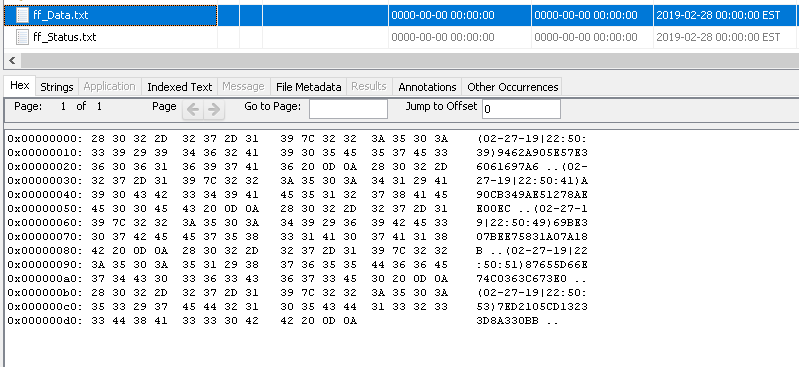
\includegraphics[width=1\textwidth]{Figures/5_results/SD_notamper.png} 
    \caption{Hex readout and excerpt of file metadata.}
    \label{fig:notamper}
\end{figure}

A quick indicator is the lack of corresponding timestamps, showing that a particular file has been edited only by a FAT library without timestamping features, as is the case for R.F.I.D. As the library used for FAT file handling was created by the design team, this specification has been met. All specifications related to the storage of data and FAT file handling have been met.

%%%%%%%%%%%%%%%%%%%%%%%%%%

\subsection{PCB}
% RELEVANT SPECS: 
% Uses a custom printed circuit board (PCB) 

All components of R.F.I.D. are located on a 4-layer PCB. This PCB was designed using the Altium design software. Next, the design was sent to JLCPCB for manufacturing. A mix of both custom-made and generic PCB footprints were used in the design of the PCB. The dimensions of the designed PCB are 61x89mm, and the thickness of the board is 1.6mm. The PCB layout as viewed from its component side is shown in Figure~\ref{fig:pcb}.

\begin{figure}[H]
    \centering
    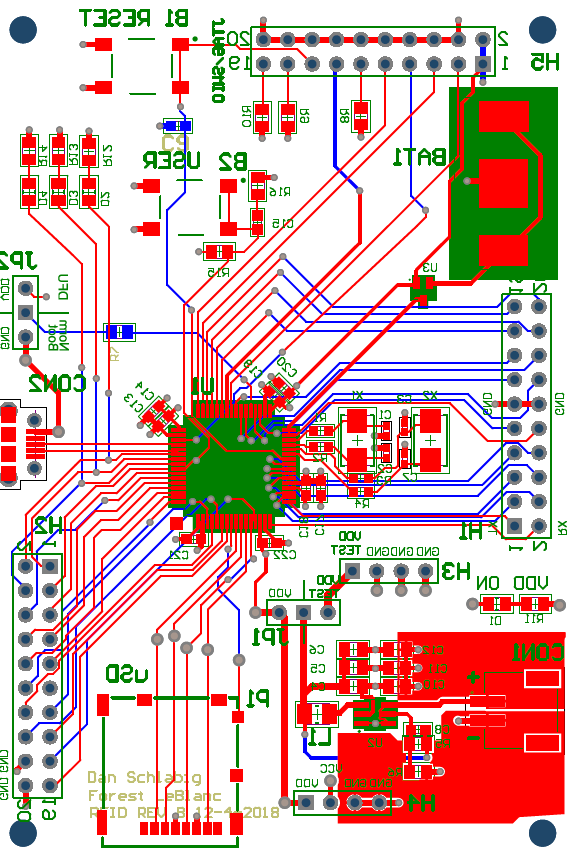
\includegraphics[scale=0.7,angle=90]{Figures/5_results/pcb_printout_3_1,2019_roughdraft.PNG} 
    \caption{PCB layout viewed from the component side.}
    \label{fig:pcb}
\end{figure}

% this part needs to be after the figure
Blue lines show traces on the bottom side of the board, while red lines show traces on the component side of the board. Four mounting holes are located on each corner of the PCB so that the PCB can be safely mounted above whatever surface that it is placed on. The project uses a custom PCB designed by the creators of R.F.I.D. Thus, the project specification for using a custom PCB is met.